\section{Ôn tập chương V}
\subsubsection{Bài tập trắc nghiệm}
\Opensolutionfile{ans}[ans/ans-1K5-3-OTC]
%BÀI 1: GIỚI HẠN DÃY SỐ%
\begin{ex}%[Đỗ Minh Phúc]%[1K5YE-2]
	Trong các giới hạn sau, giới hạn nào bằng $ 0 $?
	\choice
	{$ \lim(n^3-3n+1) $}
	{\True $ \lim\dfrac{n^2+n}{n^3+1} $}
	{$ \lim\dfrac{n^2+n+1}{4n+1} $}
	{$ \lim\dfrac{2^n-3^n}{3^n+2} $}
	\loigiai{
		Ta có $ \lim\dfrac{n^2+n}{n^3+1}=\lim\dfrac{\dfrac{1}{n}+\dfrac{1}{n^2}}{1+\dfrac{1}{n^3}}=0. $
	}
\end{ex}
\begin{ex}%[Đỗ Minh Phúc]%[1K5YE-1]
	Trong các khẳng định dưới đây, khẳng định nào \textbf{sai}?
	\choice
	{\True $\lim\limits_{n \to +\infty} q^n=0$}
	{$\lim\limits_{n \to +\infty} \dfrac{1}{n^k}=0$ với $k$ nguyên dương}
	{$\lim\limits_{n \to +\infty} \dfrac{1}{n}=0$}
	{Nếu $u_n=c$ ($c$ là hằng số) thì $\lim\limits_{n \to +\infty} u_n=\lim \limits_{n \to +\infty}c=c$}
	\loigiai{
		Ta có $\lim\limits_{n \to +\infty} q^n=0$ khi $|q|<1$; $\lim\limits_{n \to +\infty} q^n=+\infty$ khi $q>1$.}
\end{ex}

\begin{ex}%[Đỗ Minh Phúc]%[1K5BE-2]
	Tính $\lim \limits_{n \to +\infty}\dfrac{n^2+1}{2n^2+n+1}$ ta được kết quả là
	\choice
	{$\lim \limits_{n \to +\infty}\dfrac{n^2+1}{2n^2+n+1}=0$}
	{\True $\lim \limits_{n \to +\infty}\dfrac{n^2+1}{2n^2+n+1}=\dfrac{1}{2}$}
	{$\lim \limits_{n \to +\infty}\dfrac{n^2+1}{2n^2+n+1}=+\infty $}
	{$\lim \limits_{n \to +\infty}\dfrac{n^2+1}{2n^2+n+1}=1$}
	\loigiai{
		Ta có $\lim \limits_{n \to +\infty}\dfrac{n^2+1}{2n^2+n+1}=\lim \limits_{n \to +\infty}\dfrac{1+\dfrac{1}{n^2}}{2+\dfrac{1}{n}+\dfrac{1}{n^2}}=\dfrac{1}{2}$.}
\end{ex}

\begin{ex}%[Đỗ Minh Phúc]%[1K5BE-2]
	$\lim \limits_{n \to +\infty}\dfrac{2023^n+2024^n}{2025^n}$ có giá trị bằng
	\choice
	{$\dfrac{3}{5}$}
	{$+\infty$}
	{\True $0$}
	{$1$}
	\loigiai{
		Ta có $\lim \limits_{n \to +\infty}\dfrac{2023^n+2024^n}{2025^n}=\lim \limits_{n \to +\infty}\left(\dfrac{2023}{2025} \right)^n+ \lim \limits_{n \to +\infty}\left(\dfrac{2024}{2025}\right)^n=0+0=0$.}
\end{ex}

\begin{ex}%[Đỗ Minh Phúc]%[1K5BE-4]%
	Tìm $\lim \limits_{n \to +\infty}\left(\sqrt{n^2+1}-2n\right)$ ta được kết quả là
	\choice
	{\True $-\infty$}
	{$+\infty$}
	{$0$}
	{$-\dfrac{2}{3}$}
	\loigiai{
		\begin{itemize}
			\item Cách 1: $\lim\left(\sqrt{n^2+1}-2n\right)=\lim \limits_{n \to +\infty}n\left(\sqrt{1+\dfrac{1}{n^2}}-2\right)=-\infty$\\
			(vì $\lim \limits_{n \to +\infty}n=+\infty$ và $\lim\left(\sqrt{1+\dfrac{1}{n^2}}-2\right)=-1<0$).
			\item Cách 2: $\lim \limits_{n \to +\infty}\left(\sqrt{n^2+1}-2n\right)=\lim\dfrac{n^2+1-4n^2}{\sqrt{n^2+1}+2n}=\lim\dfrac{-3n+\dfrac{1}{n}}{\sqrt{1+\dfrac{1}{n^2}}+2}=-\infty$.
		\end{itemize}
	}
\end{ex}

\begin{ex}%[Đỗ Minh Phúc]%[1K5BE-5]
	Tính tổng vô hạn $S=9+3+1+\dfrac{1}{3}+\cdots +\dfrac{1}{3^{n-3}}+\cdots $
	\choice
	{$S=14$}
	{$S=15$}
	{\True $S=\dfrac{27}{2}$}
	{$S=16$}
	\loigiai{
		Dãy số $(u_n):9;3;1;\dfrac{1}{3};\cdots;\dfrac{1}{3^{n-3}};\cdots $ là một cấp số nhân lùi vô hạn với số hạng đầu $u_1=9$, công bội $q=\dfrac{1}{3}$. \\
		Do đó tổng của dãy là $S=9+3+1+\dfrac{1}{3}+\cdots +\dfrac{1}{3^{n-3}}+\cdots =\dfrac{u_1}{1-q}=\dfrac{9}{1-\dfrac{1}{3}}=\dfrac{27}{2}$.}
\end{ex}

\begin{ex}%[Đỗ Minh Phúc]%[1K5BE-1]%
	Trong các mệnh đề sau, mệnh đề nào là mệnh đề \textbf{sai}?
	\choice
	{$\lim\limits_{n\rightarrow +\infty} \dfrac{1}{n} = 0$}
	{$\lim\limits_{n\rightarrow +\infty} \dfrac{2n+1}{n-3} = 2$}
	{$\lim\limits_{n\rightarrow +\infty} (n^2-2n+1) = +\infty$}
	{\True $\lim\limits_{n\rightarrow +\infty} n^k = -\infty$ $\left( k\in \mathbb{N}^{*}\right) $}
	\loigiai{
		Ta có $\lim\limits_{n\rightarrow +\infty} n^k = +\infty$ $\left( k\in \mathbb{N}^{*} \right)$.
	}
\end{ex}

\begin{ex}%[Đỗ Minh Phúc]%[1K5KE-3]%
	Tính $\lim \limits_{n \to +\infty}n\left(\sqrt{4n^2+3}-\sqrt[3]{8n^3+n}\right)$.
	\choice
	{\True $\dfrac{2}{3}$}
	{$+\infty$}
	{$-\infty$}
	{$1$}
	\loigiai{Ta có
		\begin{align*}
			&\lim \limits_{n \to +\infty}n\left(\sqrt{4n^2+3}-\sqrt[3]{8n^3+n}\right)\\
			=&\lim \limits_{n \to +\infty}n\left[\left(\sqrt{4n^2+3}-2n\right)+\left(2n-\sqrt[3]{8n^3+n}\right)\right]\\
			=&\lim \limits_{n \to +\infty}n\left[\dfrac{3}{\sqrt{4n^2+3}+2n}+\dfrac{-n}{(2n)^2+2n\cdot\sqrt[3]{8n^3+n}+\sqrt[3]{8n^3+n}^2} \right]\\
			=&\lim \limits_{n \to +\infty}\left[\dfrac{3}{\sqrt{4+\dfrac{3}{n^2}}+2}+\dfrac{-1}{2^2+2\sqrt[3]{8+\dfrac{1}{n^2}}+\sqrt[3]{8+\dfrac{1}{n^2}}^2}\right]\\
			=&\dfrac{2}{3}.
		\end{align*}
	}
\end{ex}

\begin{ex}%[Đỗ Minh Phúc]%[1K5KE-2]
	Dãy số $(u_n)$ với $u_n=\dfrac{\sqrt{2n^3+n}+3n-1}{\sqrt{6n^3+2n^2}+n}$ có giới hạn bằng $\sqrt{\dfrac{a}{b}}$, $a>0$, $b>0$ và $\text{ƯCLN}(a,b=1)$. Hãy tính giá trị của $a^2+b^2$.
	\choice
	{$5$}
	{$40$}
	{$9$}
	{\True $10$}
	\loigiai{
		Ta có $$\lim \limits_{n \to +\infty}u_n=\lim \limits_{n \to +\infty}\dfrac{\sqrt{2n^3+n}+3n-1}{\sqrt{6n^3+2n^2}+n}=\lim \limits_{n \to +\infty}\dfrac{\sqrt{2+\dfrac{1}{n^2}}+\dfrac{3}{\sqrt{n}}-\dfrac{1}{n\sqrt{n}}}{\sqrt{6+\dfrac{2}{n}}+\dfrac{1}{\sqrt{n}}}=\sqrt{\dfrac{1}{3}}.$$
		Suy ra $a=1$, $b=3 \Rightarrow a^2+b^2=10$.}
\end{ex}

\begin{ex}%[Đỗ Minh Phúc]%[1K5BE-2]
	Tìm tất cả các giá trị thực của tham số $b$ để biểu thức $A=\lim\limits\dfrac{9-b^2n^2}{11n^2+3}<0$.
	\choice
	{$b\le 0$}
	{\True $b\ne 0$}
	{$b<0$}
	{$b>0$}
	\loigiai{Ta có $A=\lim\limits\dfrac{9-b^2n^2}{11n^2+3}=\lim\limits\dfrac{n^2\left(\dfrac{9}{n^2}-b^2\right)}{n^2\left(11+\dfrac{3}{n^2}\right)}=\lim\limits\dfrac{\dfrac{9}{n^2}-b^2}{11+\dfrac{3}{n^2}}=-\dfrac{b^2}{11}$.\\
		Yêu cầu bài toán xảy ra khi $-\dfrac{b^2}{11}<0\Leftrightarrow b^2>0\Leftrightarrow b\ne0$.}
\end{ex}

%BÀI 2: GIỚI HẠN HÀM SỐ%
\begin{ex}%[Đỗ Minh Phúc]%[1K5YF-2]
	Cho các giới hạn: $\lim \limits_{x\rightarrow x_0}f(x)=2$, $\lim \limits_{x\rightarrow x_0}g(x)=3$. Tính $M=\lim \limits_{x\rightarrow x_0}[3f(x)-4g(x)]$.
	\choice
	{$M=5$}
	{$M=2$}
	{\True $M=-6$}
	{$M=3$}
	\loigiai{
		Ta có $M=\lim \limits_{x\rightarrow x_0}[3f(x)-4g(x)]=3\lim \limits_{x\rightarrow x_0}f(x)-4\lim \limits_{x\rightarrow x_0}g(x)=6-12=-6.$
	}
\end{ex}

\begin{ex}%[Đỗ Minh Phúc]%[1K5YF-2]%
	Giá trị của $\lim\limits_{x\rightarrow -2} \left(x^3-x^2+1\right)$ bằng
	\choice
	{\True $-11$}
	{$12$}
	{$5$}
	{$0$}
	\loigiai{
		Ta có $\lim\limits_{x\rightarrow -2} \left(x^3-x^2+1\right)=\lim\limits_{x\rightarrow -2} \left((-2)^3-(-2)^2+1\right)=-11$.
	}
\end{ex}

%\begin{ex}%[Đỗ Minh Phúc]%[1K5BF-3]%
%	Giá trị của giới hạn $\lim\limits_{x \to 3} \dfrac{x^2+2x-15}{x-3}$ là
%	\choice
%	{$2$}
%	{$0$}
%	{\True $8$}
%	{$5$}
%	\loigiai{
%		Ta có $\lim\limits_{x \to 3} \dfrac{x^2+2x-15}{x-3}=\lim\limits_{x \to 3} \dfrac{(x-3)(x+5)}{x-3}=\lim\limits_{x \to 3} (x+5)=8$.}
%\end{ex}

\begin{ex}%[Đỗ Minh Phúc]%[1K5BF-6]%
	Giá trị của $\lim \limits_{x \to  - \infty } \left( \sqrt {x^2 + 5}  - x \right)$ là
	\choice
	{\True $+\infty $}
	{$-\infty $}
	{$1$}
	{$0$}
	\loigiai{
		Ta có $$\lim\limits_{x \to -\infty} \left(\sqrt{x^2+5}-x\right)=\lim\limits_{x \to -\infty} x\left(-\sqrt{1+\dfrac{5}{x^2}}-1 \right)=+\infty.$$
	}
\end{ex}

\begin{ex}%[Đỗ Minh Phúc]%[1K5BF-4]
	Giá trị của $\lim\limits_{x\to -\infty}\dfrac{2x^2-x+1}{x+2}$ là
	\choice
	{\True$-\infty $}
	{$+\infty $}
	{$-2$}
	{$1$}
	\loigiai{
		Ta có  $\lim\limits_{x\to -\infty}\dfrac{2x^2-x+1}{x+2}=\lim\limits_{x\to -\infty}\dfrac{x^2\left(2-\dfrac{1}{x}+\dfrac{1}{x^2}\right)}{x\left(1+\dfrac{2}{x}\right)}=\lim\limits_{x\to -\infty}\left[ x\cdot\dfrac{\left(2-\dfrac{1}{x}+\dfrac{1}{x^2}\right)}{1+\dfrac{2}{x}}\right]=-\infty$.
	}
\end{ex}

\begin{ex}%[Đỗ Minh Phúc]%[1K5BF-1]
	Giả sử $\displaystyle \lim_{x \rightarrow x_0} f(x) = +\infty$ và $\displaystyle \lim_{x \rightarrow x_0} g(x) = -\infty$. Ta xét các mệnh đề sau
	\begin{enumEX}[(1)]{3}
		\item $\displaystyle \lim_{x \rightarrow x_0} \left[f(x) + g(x)\right]  = 0$.
		\item $\displaystyle \lim_{x \rightarrow x_0} \dfrac{f(x)}{g(x)}  = -1$.
		\item $\displaystyle \lim_{x \rightarrow x_0} \left|f(x)\right|  = \lim\limits_{x\rightarrow x_0} \left|g(x)\right| = +\infty$.
	\end{enumEX}
	Trong các mệnh đề trên có tất cả bao nhiêu mệnh đề đúng?
	\choice
	{Có một mệnh đề đúng}
	{Có hai mệnh đề đúng}
	{Có ba mệnh đề đúng}
	{\True Không có mệnh đề nào đúng}
	\loigiai{\begin{itemize}
			\item Mệnh đề (1), (2) sai nếu ta chọn $\displaystyle \lim_{x \rightarrow x_0}f(x) =\displaystyle \lim_{x \rightarrow 1} \dfrac{3}{(x - 1)^2}$ và $\displaystyle \lim_{x \rightarrow x_0}g(x) =\displaystyle \lim_{x \rightarrow 1} \dfrac{-2}{(x - 1)^2}$. Khi đó $$\displaystyle \lim_{x \rightarrow 1} \left[f(x) + g(x)\right]  = + \infty\text{ và }\displaystyle \lim_{x \rightarrow x_0} \dfrac{f(x)}{g(x)}  = \dfrac{-3}{2}.$$
			\item Mệnh đề (3) sai vì $\displaystyle \lim_{x \rightarrow x_0} \left|f(x)\right| = +\infty$ và  $\displaystyle \lim\limits_{x\rightarrow x_0} \left|g(x)\right| = +\infty$ nhưng $\displaystyle \lim\limits_{x\rightarrow x_0} \left|f(x)\right| \neq \lim\limits_{x\rightarrow x_0} \left|g(x)\right|$.
		\end{itemize}
	}
\end{ex}

%\begin{ex}%[Đỗ Minh Phúc]%[1K5BF-3]
%	$\lim\limits_{x\to-2}\dfrac{2x^2+3x-2}{x^2-4}$ bằng
%	\choice
%	{\True $\dfrac{5}{4}$}
%	{$-\dfrac{5}{4}$}
%	{$\dfrac{1}{4}$}
%	{$2$}
%	\loigiai{
%		Ta có $\lim\limits_{x\to-2}\dfrac{2x^2+3x-2}{x^2-4}$ $=\lim\limits_{x\to-2}\dfrac{\left(2x-1\right)\left(x+2\right)}{\left(x-2\right)\left(x+2\right)}$ $=\lim\limits_{x\to-2}\dfrac{2x-1}{x-2}=\dfrac{5}{4}$.}
%\end{ex}

\begin{ex}%[Đỗ Minh Phúc]%[1K5BF-3]%
	Cho $a$ là số thực khác $0$. Tính $\lim\limits_{ x\to a} \dfrac{x^4 -a^4}{x-a}$.
	\choice
	{$a^3$}
	{\True $4a^3$}
	{$2a^3$}
	{$3a^3$}
	\loigiai{
		Ta có $\lim\limits_{ x\to a} \dfrac{x^4  -a^4}{x-a}= \lim\limits_{x \to a} \dfrac{(x-a)(x+a)\left( x^2+a^2\right) }{x-a} =\lim\limits_{x\to a} \left[\left( x^2+a^2\right) (x+a)\right]=2a^2\cdot 2a=4a^3$.
	}
\end{ex}

\begin{ex}%[Đỗ Minh Phúc]%[1K5BF-3]%
	Cho $ 2a+b=2 $ và $ \lim\limits_{x \to 2} \dfrac{ax^2+bx-4}{x-2}=5$. Khẳng định nào sau đây là đúng?
	\choice
	{$a=-1$, $b=4$}
	{$a=1$, $b=0$}
	{\True $a=\dfrac{3}{2}$, $b=-1$}
	{$a=-2$, $b=6$}
	\loigiai{
		Ta có $ 2a+b=2 \Leftrightarrow  b=2-2a $.\\
		Khi đó ta có
		\begin{eqnarray*}
			\lim\limits_{x \to 2} \dfrac{ax^2+bx-4}{x-2}=5 &\Leftrightarrow&  \lim\limits_{x \to 2} \dfrac{ax^2+(2-2a)x-4}{x-2}=5\Leftrightarrow  \lim\limits_{x \to 2} \dfrac{(ax+2)(x-2)}{x-2}=5\\
			&\Leftrightarrow&  \lim\limits_{x \to 2} (ax+2)=5\Leftrightarrow 2a+2=5\Leftrightarrow a=\dfrac{3}{2}\Rightarrow b=-1.
		\end{eqnarray*}
	} 
\end{ex}

\begin{ex}%[Đỗ Minh Phúc]%[1K5BF-5]%
	Tính $\lim\limits_{x \to 2}\dfrac{\sqrt[3]{3x+2} + x - 4}{x^2 - 3x + 2}$ ta được kết quả là
	\choice
	{$\dfrac{1}{2}$}
	{$\dfrac{1}{3}$}
	{\True $\dfrac{5}{4}$}
	{$\dfrac{1}{5}$}
	\loigiai
	{
		\allowdisplaybreaks
		\begin{eqnarray*}
			\lim\limits_{x \to 2}\dfrac{\sqrt[3]{3x+2} + x - 4}{x^2 - 3x + 2} &=& \lim\limits_{x \to 2}\dfrac{3x + 2 + (x-4)^3}{(x^2 - 3x + 2)\left[\sqrt[3]{(3x+2)^2} - (x-4)\sqrt[3]{3x+2} + (x-4)^2\right]}\\
			&=& \lim\limits_{x \to 2}\dfrac{x^3 - 12x^2 + 51x - 62}{(x^2 - 3x + 2)\left[\sqrt[3]{(3x+2)^2} - (x-4)\sqrt[3]{3x+2} + (x-4)^2\right]}\\
			&=& \lim\limits_{x \to 2}\dfrac{(x-2)(x^2 - 10x + 31)}{(x-2)(x-1)\left[\sqrt[3]{(3x+2)^2} - (x-4)\sqrt[3]{3x+2} + (x-4)^2\right]}\\
			&=& \lim\limits_{x \to 2}\dfrac{x^2 - 10x + 31}{(x-1)\left[\sqrt[3]{(3x+2)^2} - (x-4)\sqrt[3]{3x+2} + (x-4)^2\right]}\\
			&=& \dfrac{5}{4}.
		\end{eqnarray*}
		
	}
\end{ex}	

\begin{ex}%[Đỗ Minh Phúc]%[1K5BF-5]%
	Tính $\lim\limits_{x \to 0}\dfrac{\sqrt{1+x^2} - 1}{2x^3 - 3x^2}$ ta được kết quả là
	\choice
	{$-\dfrac{1}{2}$}
	{$-\dfrac{1}{4}$}
	{\True $-\dfrac{1}{6}$}
	{$-\dfrac{1}{8}$}
	\loigiai
	{
		$$\lim\limits_{x \to 0}\dfrac{\sqrt{1+x^2} - 1}{2x^3 - 3x^2} = \lim\limits_{x \to 0}\dfrac{x^2}{(2x^3 - 3x^2) \left(\sqrt{1+x^2} + 1\right)} = \lim\limits_{x \to 0}\dfrac{1}{(2x - 3) \left(\sqrt{1+x^2} + 1\right)} = -\dfrac{1}{6}.$$
	}
\end{ex}

\begin{ex}%[Đỗ Minh Phúc]%[1K5BF-5]%
	Kết quả của $\lim \limits_{x \to 0} \dfrac{\sqrt {x + 9}  + \sqrt {x + 16}  - 7}{x}$ là
	\choice
	{$\dfrac{7}{23}$}
	{\True $\dfrac{7}{24}$}
	{$\dfrac{7}{25}$}
	{$\dfrac{7}{26}$}
	\loigiai{
		\allowdisplaybreaks
		\begin{eqnarray*}
			\lim \limits_{x \to 0} \dfrac{\sqrt {x + 9}  + \sqrt {x + 16}  - 7}{x}&=&\lim \limits_{x \to 0} \dfrac{\left(\sqrt {x + 9}-3\right)+\left(\sqrt {x + 16}  - 4\right)}{x} 
			=\lim \limits_{x \to 0}\left[\dfrac{\sqrt {x + 9}-3}{x}+\dfrac{\sqrt{x+16}-4}{x}\right]\\
			&=&\lim \limits_{x \to 0}\left[\dfrac{x}{x\left(\sqrt {x + 9}+3\right)}+\dfrac{x}{x\left(\sqrt{x+16}+4\right)}\right]\\
			&=&\lim \limits_{x \to 0}\left[\dfrac{1}{\sqrt {x + 9}+3}+\dfrac{1}{\sqrt{x+16}+4}\right]\\
			&=&\dfrac{1}{6}+\dfrac{1}{8}
			=\dfrac{7}{24}.
		\end{eqnarray*}
	}
\end{ex}

\begin{ex}%[Đỗ Minh Phúc]%[1K5BF-5]%
	Giới hạn $\lim\limits_{x \to -\infty} \left(\sqrt{x^2-4x}-\sqrt{x^2-x}\right)$ bằng
	\choice
	{$-\dfrac{3}{2}$}
	{$\dfrac{1}{2}$}
	{\True $\dfrac{3}{2}$}
	{$-\dfrac{1}{2}$}
	\loigiai{
		Ta có 
		$$\lim\limits_{x \to -\infty} \left(\sqrt{x^2-4x}-\sqrt{x^2-x}\right)=\lim\limits_{x \to -\infty} \dfrac{-3x}{\sqrt{x^2-4x}+\sqrt{x^2-x}}=\lim\limits_{x \to -\infty} \dfrac{3x}{x\left(\sqrt{1-\dfrac{4}{x}}+\sqrt{1-\dfrac{1}{x}}\right)}=\dfrac{3}{2}.$$}
\end{ex}

\begin{ex}%[Đỗ Minh Phúc]%[1K5BF-5]%
	Giới hạn $ \lim\limits_{x\to +\infty}\dfrac{2x-3a}{3x+2a} $ (với $ a $ là tham số) có giá trị bằng
	\choice
	{$2$}
	{$-1$}
	{$\dfrac{3}{2}$}
	{\True $\dfrac{2}{3}$}
	\loigiai{
		Ta có $ \lim\limits_{x\to +\infty}\dfrac{2x-3a}{3x+2a} =\lim\limits_{x\to +\infty}\dfrac{2-\dfrac{3a}{x}}{3+\dfrac{2a}{x}}=\dfrac{2}{3}$.
	}
\end{ex}

\begin{ex}%[Đỗ Minh Phúc]%[1K5BF-5]
	Tìm giới hạn $I= \lim\limits_{x\to +\infty}\left( x+1 -\sqrt{x^2-x-2}\right)$.
	\choice
	{\True $I=\dfrac{3}{2}$}
	{$I=\dfrac{1}{2}$}
	{$I=\dfrac{17}{11}$}
	{$I=\dfrac{46}{31}$}
	\loigiai{
		\begin{align*}
			I= \lim\limits_{x\to +\infty}\left( x+1 -\sqrt{x^2-x-2}\right)&=\lim\limits_{x\to +\infty}\dfrac{\left( x+1 -\sqrt{x^2-x-2}\right)\left( x+1 +\sqrt{x^2-x-2}\right)}{x+1 +\sqrt{x^2-x-2}}\\
			&= \lim\limits_{x\to +\infty}\dfrac{(x+1)^2-\left( x^2-x-2\right) }{x+1 +\sqrt{x^2-x-2}}\\
			&= \lim\limits_{x\to +\infty}\dfrac{3x+3}{x+1 +\sqrt{x^2-x-2}}\\
			&=\lim\limits_{x\to +\infty}\dfrac{x\left(3+\dfrac{3}{x}\right)}{x\left(1+\dfrac{1}{x}+\sqrt{1-\dfrac{1}{x}-\dfrac{2}{x^2}}\right)}\\
			&=\lim\limits_{x\to +\infty}\dfrac{3+\dfrac{3}{x}}{1+\dfrac{1}{x}+\sqrt{1-\dfrac{1}{x}-\dfrac{2}{x^2}}}=\dfrac{3}{2}.
		\end{align*}
	}
\end{ex}

\begin{ex}%[Đỗ Minh Phúc]%[1K5BF-5]%
	Giá trị của giới hạn $\lim\limits_{x \to +\infty} \left(\sqrt{x^2+x+1}-\sqrt{x^2-x+1}\right)$ là
	\choice
	{$0$}
	{\True $1$}
	{$2$}
	{$3$}
	\loigiai{
		Ta có
		\allowdisplaybreaks
		\begin{eqnarray*}
			\lim\limits_{x \to +\infty} \left(\sqrt{x^2+x+1}-\sqrt{x^2-x+1}\right)&=& \lim\limits_{x \to +\infty} \dfrac{2x}{\sqrt{x^2+x+1}+\sqrt{x^2-x+1}}\\
			& =& \lim\limits_{x \to +\infty}
			\dfrac{2}{\sqrt{1+\dfrac{1}{x}+\dfrac{1}{x^2}}+\sqrt{1-\dfrac{1}{x}+\dfrac{1}{x^2}}}=1.
		\end{eqnarray*}
		
	}
\end{ex}

\begin{ex}%[Đỗ Minh Phúc]%[1K5KF-5]%
	Cho $\lim\limits_{x\to 1}\dfrac{\sqrt{x+3}-2}{x^2-1}=\dfrac{a}{b}$, trong đó $\dfrac{a}{b}$ là phân số tối giản. Tổng $a+b$ có giá trị bằng
	\choice
	{\True $9$}
	{$8$}
	{$7$}
	{$6$}
	\loigiai{
		Ta có \begin{eqnarray*}
			\lim\limits_{x\to 1}\dfrac{\sqrt{x+3}-2}{x^2-1}&=&\lim\limits_{x\to 1}\dfrac{\left(\sqrt{x+3}-2\right)\left(\sqrt{x+3}+2\right)}{(x^2-1)\left(\sqrt{x+3}+2\right)}\\
			&=&\lim\limits_{x\to 1}\dfrac{x+3-4}{(x-1)(x+1)\left(\sqrt{x+3}+2\right)}\\
			&=&\lim\limits_{x\to 1}\dfrac{x-1}{(x-1)(x+1)\left(\sqrt{x+3}+2\right)}\\
			&=&\lim\limits_{x\to 1}\dfrac{1}{(x+1)\left(\sqrt{x+3}+2\right)}\\
			&=&\dfrac{1}{(1+1)\left(\sqrt{1+3}+2\right)}=\dfrac{1}{8}.
		\end{eqnarray*}
		Từ đó suy ra $a+b=1+8=9$.
	}
\end{ex}

\begin{ex}%[Đỗ Minh Phúc]%[1K5BF-7]
	Tính $I =\lim\limits_{x \to 1^+} \dfrac{3x+2}{1-x}$ ta được kết quả là
	\choice
	{$I=+\infty$}
	{\True $I=-\infty$}
	{$I=0$}
	{$I=-3$}
	\loigiai{
		Ta có $\lim\limits_{x \to 1^+} (3x+2)=5$, $\lim\limits_{x \to 1^+} (1-x)=0$ và $1-x<0$ khi $x>1$. \\
		Nên $\lim\limits_{x \to 1^+} \dfrac{3x+2}{1-x}=-\infty$.}
\end{ex}

\begin{ex}%[Đỗ Minh Phúc]%[1K5BF-7]%
	Tính $\lim\limits_{x\to 3^+}\dfrac{-x^2+5}{x-3}$ ta được kết quả là
	\choice
	{\True $-\infty$}
	{$+\infty$}
	{$1$}
	{Không tồn tại}
	\loigiai
	{
		Ta có $\lim\limits_{x\to 3^+}(-x^2+5)=-4<0,\ \lim\limits_{x\to 3^+}(x-3)=0$ và $x-3>0,\forall x>3$.\\ Do đó $\lim\limits_{x\to 3^+}\dfrac{-x^2+5}{x-3}=-\infty$.
	}
\end{ex}

\begin{ex}%[Đỗ Minh Phúc]%[1K5BF-7]%
	Tính $\lim\limits_{x\to (-2)^+}\dfrac{\left| x^2-4\right| }{x+2}$ ta được kết quả là
	\choice
	{$1$}
	{\True $4$}
	{$2$}
	{$3$D}
	\loigiai
	{
		Ta có $\lim\limits_{x\to -2^+}\dfrac{|x^2-4|}{x+2}=\lim\limits_{x\to -2^+}\dfrac{4-x^2}{x+2}=\lim\limits_{x\to -2^+}(2-x)=4$.
	}
\end{ex}

\begin{ex}%[Đỗ Minh Phúc]%[1K5BF-7]
	Tính $\lim\limits_{x\to 1} \dfrac{2x+1}{x-1}$ ta được kết quả là
	\choice
	{$0$}
	{$+\infty$}
	{$-\infty$}
	{\True Không tồn tại}
	\loigiai
	{
		Ta có $\lim\limits_{x\to 1^{-}}(2x+1)=3>0$; $\lim\limits_{x\to1^{-}}(x-1)=0$ và $x-1<0$, $\forall x<1$ nên $\lim\limits_{x\to 1^{-}}\dfrac{2x+1}{x-1}=-\infty$.\\
		Tương tự, ta cũng có $\lim\limits_{x\to 1^{+}}(2x+1)=3>0$; $\lim\limits_{x\to1^{+}}(x-1)=0$ và $x-1>0$, $\forall x>1$ nên $\lim\limits_{x\to 1^{+}}\dfrac{2x+1}{x-1}=+\infty$.\\
		Vì $\lim\limits_{x\to 1^{-}}\dfrac{2x+1}{x-1}\ne \lim\limits_{x\to 1^{+}}\dfrac{2x+1}{x-1}$ nên không tồn tại $\lim\limits_{x\to 1} \dfrac{2x+1}{x-1}$.
	}
\end{ex}

\begin{ex}%[Đỗ Minh Phúc]%[1K5BF-3]%
	Giá trị của $\lim\limits_{x \to a} \dfrac{x^2 - \left( a + 1\right)x + a}{x^3 - a^3}$ $(a\ne 0)$ là
	\choice
	{$ + \infty $}
	{$\dfrac{a + 1}{3a^2}$}
	{$\dfrac{a - 1}{3a}$}
	{\True $\dfrac{a - 1}{3a^2}$}
	\loigiai{Ta có 
		$$\lim\limits_{x \to a} \dfrac{x^2-(a+1)x+a}{x^3-a^3}=\lim\limits_{x \to a} \dfrac{(x-a)(x-1)}{(x-a)(x^2+ax+a^2)}=\dfrac{a-1}{3a^2}.$$
	}
\end{ex}

%BÀI 3: HÀM SỐ LIÊN TỤC%
\begin{ex}%[Đỗ Minh Phúc]%[1K5YG-1]%
	Cho hàm số $ y=f(x) $ liên tục trên khoảng $ (a;b) $. Hàm số $ y=f(x) $ liên tục trên đoạn $ [a;b] $ nếu điều kiện nào sau đây xảy ra?
	\choice
	{$\lim\limits_{x \to {a^ - }} f\left( x \right) = f\left( a \right),\ \lim\limits_{x \to {b^ + }} f\left( x \right) = f\left( b \right)$}
	{\True $\lim\limits_{x \to {a^ + }} f\left( x \right) = f\left( a \right),\ \lim\limits_{x \to {b^ - }} f\left( x \right) = f\left( b \right)$}
	{$\lim\limits_{x \to {a^ - }} f\left( x \right) = a,\ \lim\limits_{x \to {b^ + }} f\left( x \right) = b$}
	{$\lim\limits_{x \to {a^ + }} f\left( x \right) = a,\ \lim\limits_{x \to {b^ - }} f\left( x \right) = b$}
	\loigiai{ Hàm số $ y=f(x) $ được gọi là liên tục trên đoạn $ [a;b] $ nếu nó liên tục trên khoảng $ (a;b) $ và $\lim\limits_{x \to {a^ + }} f\left( x \right) = f\left( a \right),\ \lim\limits_{x \to {b^ - }} f\left( x \right) = f\left( b \right)$.
	}
\end{ex}

\begin{ex}%[Đỗ Minh Phúc]%[1K5YG-3]
	Trong các hàm số sau, hàm số nào liên tục tại điểm $x=0$?
	\choice
	{$y=\dfrac{x^2-2x+3}{x}$}
	{\True $y=x^3-2x^2-x+1$}
	{$y=\cot x$}
	{$y=\sqrt{2x^2-1}$}
	\loigiai{
		\begin{itemize}
			\item Hàm số $y=\dfrac{x^2-2x+3}{x}$ có tập xác định là $\mathscr{D}=\mathbb{R}\setminus\{0\}$ nên bị gián đoạn tại điểm $x=0$.
			\item Hàm số $y=x^3-2x^2-x+1$ là hàm đa thức, liên tục trên $\mathbb{R}$ nên nó liên tục tại điểm $x=0$.
			\item Hàm số $y=\cot x$ có tập xác định là $\mathscr{D}=\mathbb{R}\setminus\{k\pi,k\in\mathbb{Z}\}$ nên bị gián đoạn tại điểm $x=0$.
			\item Hàm số $y=\sqrt{2x^2-1}$ có tập xác định là $\mathscr{D}=\left(-\infty;-\dfrac{\sqrt{2}}{2}\right]\cup\left[\dfrac{\sqrt{2}}{2};+\infty\right) $ nên bị gián đoạn tại điểm $x=0$.
		\end{itemize}
	}
\end{ex}

\begin{ex}%[Đỗ Minh Phúc]%[1K5YG-1]%
	Chọn khẳng định đúng trong các khẳng định sau
	\choice
	{\True Nếu hàm số $f(x)$ liên tục trên $[a;b]$ và $f(a)f(b)<0$ thì phương trình $f(x)=0$ có ít nhất một nghiệm trên $(a;b)$}
	{Nếu phương trình $f(x)=0$ có nghiệm trong khoảng $(a;b)$ thì hàm số $f(x)$ liên tục trên $[a;b]$ và $f(a)f(b)<0$}
	{Nếu hàm số $f(x)$ liên tục trên $[a;b]$ và $f(a)f(b)<0$ thì phương trình $f(x)=0$ có đúng một nghiệm trên $(a;b)$}
	{Nếu hàm số $f(x)$ liên tục trên $[a;b]$ và $f(a)f(b)<0$ thì phương trình $f(x)=0$ có một nghiệm trên $[a;b]$}
	\loigiai{Định lí về sự tồn tại nghiệm của phương trình trên một khoảng.
	}
\end{ex}

\begin{ex}%[Đỗ Minh Phúc]%[1K5BG-2]%
	\immini{Cho hàm số $y=f(x)$ có đồ thị dưới đây, trên khoảng $(-2;3)$ hàm số gián đoạn tại điểm nào?
		\choice
		{$x=0$}
		{\True $x=1$}
		{$x=2$}
		{$x=3$}}{	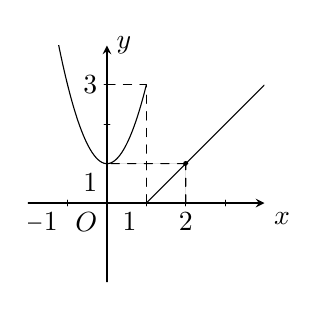
\begin{tikzpicture}[line join=round, line cap=round, >=stealth, scale=0.5]
			\draw[->](-2,0)--(4,0) node[below right] {$x$};;
			\draw[->](0,-2)--(0,4) node[right] {$y$};
			\clip (-2,-2) rectangle (4,4);
			\foreach \x in {-1,...,3}
			\draw[shift={(\x,0)},color=black] (0pt,2pt) -- (0pt,-2pt);
			\foreach \y in {0,...,3}
			\draw[shift={(0,\y)},color=black] (2pt,0pt) -- (-2pt,0pt);
			\draw[samples=100,smooth,domain=-2:1] plot(\x,{2*(\x)^2+1});
			\draw[fill=black,dashed](2,0)node[below]{$2$}--(2,1)circle(1.5pt)--(0,1)node[below left]{$1$};
			\draw[dashed] (1,0)node [below left]{$1 $}--(1,3)--(0,3)node [left]{$3$}  (0,0)node [below left]{$ O $} (-1,0)node[below left]{$-1$};
			\draw[smooth,samples=100,domain=1:4] 
			plot(\x,{\x-1});
	\end{tikzpicture}}
	\loigiai{ Dựa vào đồ thị hàm số ta thấy $ \lim \limits_{x \to 1^{-}} f(x)=3 $ và  $ \lim \limits_{x \to 1^{+}} f(x)=0 $, suy ra $\lim \limits_{x \to 1^-} f(x) \ne \lim \limits_{x \to 1^+} f(x) $. Do đó hàm số gián đoạn tại $x=1$.}
\end{ex}

\begin{ex}%[Đỗ Minh Phúc]%[1K5BG-3]%
	Cho hàm số $f(x)=\heva{&\dfrac{x^2-3x+2}{x-1}&,\text{khi }x>1\\&2x+1 &,\text{khi } x\le 1}$. Chọn khẳng định đúng.
	\choice
	{Hàm số $f(x)$ liên tục tại điểm $x=1$}
	{Hàm số $f(x)$ gián đoạn tại điểm $x=1$ vì $\lim\limits_{x\to 1}f(x)\ne f(1)$}
	{\True Hàm số $f(x)$ gián đoạn tại điểm $x=1$ vì không tồn tại $\lim\limits_{x\to 1}f(x)$}
	{Hàm số $f(x)$ không xác định tại $x=1$}
	\loigiai{
		Ta có
		\begin{itemize}
			\item $\lim\limits_{x\to 1^+}f(x)=\lim\limits_{x\to 1^+}\dfrac{x^2-3x+2}{x-1}=\lim\limits_{x\to 1^+}\dfrac{(x-1)(x-2)}{x-1}=\lim\limits_{x\to 1^+}(x-2)=-1$.
			\item $\lim\limits_{x\to 1^-}f(x)=\lim\limits_{x\to 1^-}(2x+1)=3$.
		\end{itemize}
		Vì $\lim\limits_{x\to 1^+}f(x)\ne \lim\limits_{x\to 1^-}f(x)$ nên không tồn tại $\lim\limits_{x\to 1}f(x)$.\\
		Do đó hàm số gián đoạn tại điểm $x=1$ vì không tồn tại $\lim\limits_{x\to 1}f(x)$.
	}
\end{ex}

\begin{ex}%[Đỗ Minh Phúc]%[1K5BG-4]%
	Hàm số nào sau đây liên tục trên $\mathbb{R}$?
	\choice{$y=\cos{\dfrac{3}{x}}$}
	{$y=\cot 3x$}
	{\True$y = \dfrac{1-x}{x^2 + 4}$}
	{$ y = \sqrt{x+2}$}
	\loigiai{
		\begin{itemize}
			\item Hàm số $ y = \cos{\dfrac{3}{x}}$ có tập xác định là $\mathscr{D}=\mathbb{R}\setminus\{0\}$ nên không liên tục trên $\mathbb{R}$.
			\item Hàm số $y=\cot 3x$ có tập xác định là $\mathscr{D}=\mathbb{R}\setminus\left\lbrace k\dfrac{\pi}{3},k\in\mathbb{Z}\right\rbrace $ nên không liên tục trên $\mathbb{R}$.
			\item Hàm số $y = \dfrac{1-x}{x^2 + 4}$ là hàm sơ cấp nên có tập xác định $ \mathbb{R} $ nên liên tục trên $ \mathbb{R} $.
			\item Hàm số $y=\sqrt{x+2}$ có tập xác định là $\mathscr{D}=\left[-2;+\infty\right)$ nên không liên tục trên $\mathbb{R}$.
		\end{itemize}
	}
\end{ex}

\begin{ex}%[Đỗ Minh Phúc]%[1K5BG-4]%
	Cho hàm số $f(x)= \dfrac{x^2+3}{x^2-5x+6}.$ Hàm số $f(x)$ liên tục trên khoảng nào dưới đây?
	\choice
	{\True $(2;3)$}
	{$(-3;3)$}
	{$(-3;+ \infty)$}
	{$(- \infty ;3)$}
	\loigiai
	{ Hàm số xác định trên tập $\mathscr{D} = (- \infty ;2) \cup (2;3) \cup (3;+\infty)$, suy ra hàm số liên tục trên khoảng $(2;3).$
	}
\end{ex}

\begin{ex}%[Đỗ Minh Phúc]%[1K5BG-4]%
	Cho hàm số $y=\dfrac{x+4}{x-3}$. Mệnh đề nào sau đây là đúng?
	\choice
	{Hàm số liên tục tại $x=3$}
	{Hàm số liên tục trên $(-\infty;+\infty)$}
	{Hàm số liên tục tại $x=2$ và $x=3$}
	{\True Hàm số liên tục trên $(-\infty;3)$ và $(3;+\infty)$}
	\loigiai{
		Với $x_0 \neq 3$, ta có $\displaystyle \lim_{x \to x_0} f(x) = f(x_0)$ suy ra hàm số  liên tục $(-\infty;3)$ và $(3;+\infty)$. 
	}
\end{ex}

\begin{ex}%[Đỗ Minh Phúc]%[1K5BG-5]%
	Cho hàm số $y=f(x)= \heva{&\dfrac{x^3 - x^2}{x - 1} & \text{khi } x > 1 \\&n & \text{khi } x = 1 \\& mx + 1 & \text{khi } x < 1}$. Biết hàm số $ f(x) $ liên tục tại $x_0 = 1$. Giá trị của $ m$, $n$ là
	\choice
	{\True $n=1$, $m=0$}
	{$n=0$, $m=1$}
	{$n=m=1$}
	{$n=-1$, $m=0$}
	\loigiai{
		Ta có
		\begin{itemize}
			\item $\lim\limits_{x \to 1^+} f(x)=\lim\limits_{x \to 1^+} \dfrac{x^3-x^2}{x-1}=\lim\limits_{x \to 1^+}x^2=1$.
			\item $\lim\limits_{x \to 1^-}f(x)=\lim\limits_{x \to 1^-} (mx+1)=m+1$.
			\item $f(1) = n$.
		\end{itemize}
		Do hàm số $f(x)$ liên tục tại $x=1$ nên ta có $$\lim\limits_{x \to 1^-} f(x) = \lim\limits_{x \to 1^+} f(x) = f(1) \Leftrightarrow m+1 = 1 = n.$$
		Suy ra $n=1$, $m=0$.	
	}
\end{ex}

\begin{ex}%[Đỗ Minh Phúc]%[1K5BG-5]%
	Cho hàm số $f(x)=\heva{x^3+x^2+7 & \text{ khi }x\neq -1&\\2x+m-1&\text{ khi } x=-1}$. Tìm $m$ để hàm số liên tục tại điểm $x_0=-1$.
	\choice
	{$m=12$}
	{$m=8$}
	{$m=-10$}
	{\True $m=10$}
	\loigiai{
		Ta có $\lim\limits_{x\to -1} (x^3+x^2+7)=7$ và $f(-1)=m-3$.\\
		Để hàm số liên tục tại điểm $x_0=-1$ thì $m-3=7\Leftrightarrow m=10$.
	}
\end{ex}

\begin{ex}%[Đỗ Minh Phúc]%[1K5BG-7]%
	Tìm tất cả các giá trị thực của $m$ để phương trình $m(x-1)^3(x-2)+2x-3=0$ vô nghiệm.
	\choice
	{$\forall m\in \mathbb{R}$}
	{$m=1$}
	{\True Không có giá trị $m$}
	{$m=0$}
	\loigiai{
		Đặt $f(x)=m(x-1)^3(x-2)+2x-3$ xác định và liên tục trên $\mathbb{R}$. \\
		Ta có $f(1)=-1$, $f(2)=1 \Rightarrow f(1)\cdot f(2)<0,\forall m\in \mathbb{R}$ suy ra phương trình luôn có nghiệm $\forall m\in \mathbb{R}$.}
\end{ex}

\begin{ex}%[Đỗ Minh Phúc]%[1K5BG-7]%
	Phương trình nào dưới đây có nghiệm trong khoảng $\left(0;1\right)$?
	\choice
	{$2x^2-3x+4=0$}
	{${\left(x-1\right)}^5-x^7-2=0$}
	{$3x^4-4x^2+5=0$}
	{\True $3x^{2024}-8x+4=0$}
	\loigiai{
		Xét hàm số $f(x)=3x^{2024}-8x+4=0$ liên tục trên $\mathbb{R}$.\\
		Ta có $f(0)=4$; $f(1)=-1\Rightarrow f(0)\cdot f(1)=-4<0$ suy ra phương trình có ít nhất một nghiệm thuộc khoảng $\left(0;1\right)$.}
\end{ex}

\begin{ex}%%[Đỗ Minh Phúc]%[1K5BG-3]%
	Hàm số nào sau đây gián đoạn tại $x=-\sqrt{2}$ ?
	\choice
	{$y=\cos x$}
	{\True $y=\dfrac{3x+2\sqrt{2}}{x^2-2}$}
	{$y=x+\sqrt{2}$}
	{$y=\tan x$}
	\loigiai{
		Ta có $\lim\limits_{x \to \left(-\sqrt{2}\right)^-} \dfrac{3x+2\sqrt{2}}{x^2-2}=-\infty$ và $\lim\limits_{x \to \left(-\sqrt{2}\right)^+} \dfrac{3x+2\sqrt{2}}{x^2-2}=+\infty$ nên hàm số $y=\dfrac{3x+2\sqrt{2}}{x^2-2}$ gián đoạn tại $x=-\sqrt{2}$.}
\end{ex}

\begin{ex}%[Đỗ Minh Phúc]%[1K5BG-5]%
	Tìm $m$ để hàm số $f(x)= \heva{&\dfrac{\sqrt{x^2+1}-1}{x}&\text{ khi }x \ne 0\\& 2m+2&\text{ khi }x=0}$ liên tục tại $x=0$.
	\choice
	{$m=2$}
	{$m=1$}
	{\True $m=-1$}
	{$m=-2$}
	\loigiai{
		Ta có $\lim\limits_{x \to 0} f(x)=\lim\limits_{x \to 0} \dfrac{\sqrt{x^2+1}-1}{x}=\lim\limits_{x \to 0} \dfrac{x}{\sqrt{x^2+1}+1}=0$, $f(0)=2m+2$. \\
		Hàm số liên tục tại $x=0 \Leftrightarrow \lim\limits_{x \to 0} f(x)=f(0) \Leftrightarrow 2m+2=0 \Leftrightarrow m=-1$.}
\end{ex}

\begin{ex}%[Đỗ Minh Phúc]%[1K5BG-4]%
	Hàm số nào sau đây \textbf{không} liên tục trên $\mathbb{R}$?
	\choice
	{$f(x)=\dfrac{x+1}{x^2+1}$}
	{\True $f(x)=\dfrac{x+1}{x-1}$}
	{$f(x)=\sin \left(x-\dfrac{\pi}{5}\right)$}
	{$f(x)=x^3-2x^2+x-7$}
	\loigiai{
		\begin{itemize}
			\item Hàm số $f(x)=\dfrac{x+1}{x^2+1}$ là hàm sơ cấp nên có tập xác định $ \mathbb{R} $ nên liên tục trên $ \mathbb{R} $.
			\item Hàm số $f(x)=\dfrac{x+1}{x-1}$ có tập xác định $\mathbb{R} \setminus \{1\}$ nên hàm số không liên tục trên $\mathbb{R}$.
			\item Hàm số $\sin \left(x-\dfrac{\pi}{5}\right)$ là hàm sơ cấp nên có tập xác định $ \mathbb{R} $ nên liên tục trên $ \mathbb{R} $.
			\item Hàm số $f(x)=x^3-2x^2+x-7$ là hàm đa thức nên liên tục trên $ \mathbb{R} $.
		\end{itemize}	
	}
\end{ex}

\begin{ex}%[Đỗ Minh Phúc]%[1K5BG-3]%
	Cho hàm số $f(x)$ chưa xác định tại $x=0$, $f(x)=\dfrac{x^3+2x^2}{x^2}$. Để hàm số $f(x)$ liên tục tại $x=0$ thì phải gán cho $f(0)$ giá trị bằng bao nhiêu?
	\choice
	{$3$}
	{\True $2$}
	{$1$}
	{$0$}
	\loigiai{
		Ta có $\lim\limits_{x\rightarrow 0}f(x)=\lim\limits_{x\rightarrow 0}\dfrac{x^3+2x^2}{x^2}=\lim\limits_{x\rightarrow 0}(x+2)=2$.\\
		Do đó, để hàm số $f(x)$ liên tục tại $x=0$ thì phải gán cho $f(0)=2$.
	}
\end{ex}

\begin{ex}%[Đỗ Minh Phúc]%[1K5KG-5]%
	Cho hàm số $f(x)=\heva{&\dfrac{3-x}{\sqrt{x+1}-2} &\text{ nếu } x\ne 3\\&m&\text{ nếu } x=3}$.
	Hàm số đã cho liên tục tại $x=3$ khi $m$ bằng
	\choice
	{$1$}
	{$4$}
	{$-1$}
	{\True $-4$}
	\loigiai{Ta có $\underset{x\to 3}{\mathop {\lim}} \dfrac{3-x}{\sqrt {x+1}-2}=\underset{x\to 3}{\mathop{\lim}} \dfrac{(3-x)(\sqrt{x+1}+2)}{x-3}=\underset{x\to 3}{\mathop{\lim}}(-\sqrt {x+1}-2)=-4$.\\
		Hàm số liên tục tại $ x=3 $ khi và chỉ khi $\underset{x\to 3}{\mathop {\lim}} \dfrac{3-x}{\sqrt {x+1}-2}=f(3) \Leftrightarrow -4=m \Leftrightarrow m=-4  $. }
\end{ex}

\begin{ex}%[Đỗ Minh Phúc]%[1K5KG-5]%
	Cho hàm số $f(x)=\heva{&\dfrac{x^2-16}{x-4}\; &\text{khi}\; x\ne 4\\&ax-1 \; &\text{khi}\; x= 4}$. Tập hợp các giá trị của $a$ để hàm số liên tục tại $x=4$ là
	\choice
	{\True $\left\{\dfrac{9}{4}\right\}$}
	{$\left\{-\dfrac{9}{4}\right\}$}
	{$\left\{8\right\}$}
	{$\left\{0\right\}$}
	\loigiai{
		Ta có: 
		\begin{itemize}
			\item $f(4)=a\cdot 4-1=4a-1$.
			\item $\lim\limits_{x\rightarrow 4}f(x)=\lim\limits_{x\rightarrow 4}\dfrac{x^2-16}{x-4}=\lim\limits_{x\rightarrow 4}\dfrac{(x-4)(x+4)}{x-4}=\lim\limits_{x\rightarrow 4}(x+4)=8$.
		\end{itemize}
		Do đó, điều kiện cần và đủ để hàm số đã cho liên tục tại $x=4$ là 
		$$\lim\limits_{x\rightarrow 4}f(x)=f(4)\Leftrightarrow 8=4a-1\Leftrightarrow a=\dfrac{9}{4}.$$
	}
\end{ex}

\begin{ex}%[Đỗ Minh Phúc]%[1K5GG-5]%
	Tìm $m$ để hàm số $f(x)=\heva{& \dfrac{\sqrt[3]{x-2}+2 x-1}{x-1} & \text { khi } x \neq 1 \\ & 3m-2 & \text { khi } x=1}$ liên tục trên $\mathbb{R}$.
	\choice
	{$m=1$}
	{\True $m=\dfrac{4}{3}$}
	{$m=2$}
	{$m=0$}
	\loigiai
	{
		Với $x\neq 1$, ta có $f(x)=\dfrac{\sqrt[3]{x-2}+2 x-1}{x-1}$ nên hàm số liên tục trên các khoảng $(-\infty;1)$ và $(1;+\infty)$.\\
		Do đó, để hàm số liên tục trên $\mathbb{R}$ thì hàm số liên tục tại $x=1$.\\
		Ta có $f(1)=3 m-2$.\\
		Ta có 
		\allowdisplaybreaks
		\begin{eqnarray*}
			\lim\limits_{x \rightarrow 1} f(x)
			& = & \lim\limits_{x \rightarrow 1} \dfrac{\sqrt[3]{x-2}+2 x-1}{x-1} \\
			& = & \lim\limits_{x \rightarrow 1}\left[1+\dfrac{x^{3}+x-2}{(x-1)\left(x^{2}-x \sqrt[3]{x-2}+\sqrt[3]{(x-2)^{2}}\right)}\right]\\
			& = & \lim\limits_{x \rightarrow 1}\left[1+\dfrac{x^{2}+x+2}{x^{2}-x \sqrt[3]{x-2}+\sqrt[3]{(x-2)^{2}}}\right]=2.
		\end{eqnarray*}
		Nên hàm số liên tục tại $x=1$ khi và chỉ khi 
		$\lim\limits_{x \rightarrow 1} f(x)=f(1) \Leftrightarrow 3 m-2=2 \Leftrightarrow m=\dfrac{4}{3}$.\\
		Vậy $m=\dfrac{4}{3}$.
	}
\end{ex}
\begin{ex}%%[Đỗ Minh Phúc]%[1K5GG-4]%
	Có bao nhiêu giá trị thực của tham số $m$ để hàm số $f\left(x\right)=\heva{&m^2x^2&\text{ khi }x\le 2\\&(1-m)x&\text{ khi }x>2}$ liên tục trên $\mathbb{R}$?
	\choice
	{$0$}
	{\True $2$}
	{$3$}
	{$4$}
	\loigiai{
		Ta có hàm số luôn liên tục $\forall x\ne 2$ .\newline
		Tại $x=2$ , ta có
		\begin{itemize}
			\item $\lim\limits_{x\to{2^+}}f\left(x\right)=\lim\limits_{x\to{2^-}}\left(1-m\right)x=\left(1-m\right)\cdot 2=2-2m$;
			\item $\lim\limits_{x\to{2^-}}f\left(x\right)=\lim\limits_{x\to{2^-}}\left(m^2x^2\right)=4m^2$;
			\item $f\left(2\right)=4m^2$.
		\end{itemize}
		Hàm số liên tục tại $x=2$ khi và chỉ khi
		$$\lim\limits_{x\to{2^+}}f\left(x\right)=\lim\limits_{x\to{2^-}}f\left(x\right)=f\left(2\right)\Leftrightarrow 4m^2=2-2m\Leftrightarrow 4m^2+2m-2=0\Leftrightarrow\hoac{&m=\dfrac{1}{2}\\&m=-1.}$$
		Vậy có hai giá trị của $m$.}
\end{ex}
\Closesolutionfile{ans}
\begin{indapan}{10}
	{ans/ans-1K5-3-OTC}
\end{indapan}